% Copyright (C) 2005-2015 Airbus - EDF - IMACS - Phimeca
% Permission is granted to copy, distribute and/or modify this document
% under the terms of the GNU Free Documentation License, Version 1.2
% or any later version published by the Free Software Foundation;
% with no Invariant Sections, no Front-Cover Texts, and no Back-Cover
% Texts.  A copy of the license is included in the section entitled "GNU
% Free Documentation License".
\renewcommand{\nomfichier}{docref_C311_TransIso_Rosenblatt}
\renewcommand{\titrefiche}{Rosenblatt Transformation}

\Header

\MathematicalDescription{
  \underline{\textbf{Goal}} \vspace{2mm}

  The Rosenblatt transformation is an isoprobabilistic transformation (refer to  \otref{docref_C311_TransIso}{Isoprobabilistic Transformation}) which is used under the following context : $\vect{X}$ is the input random vector,  $F_i$ the cumulative density functions of its components and $C$ its copula, without no condition on its type.\\

  Let us denote by $\vect{d}$ a determinist vector, $g(\vect{X}\,,\,\vect{d})$ the limit state function of the model, $\cD_f = \{\vect{X} \in \Rset^n \, / \, g(\vect{X}\,,\,\vect{d}) \le 0\}$ the  event considered here and {g(\vect{X}\,,\,\vect{d}) = 0} its boundary.\\

  One way to evaluate the probability content of the event $\cD_f$:
  \begin{equation}\label{PfX2}
    P_f = \Prob{g(\vect{X}\,,\,\vect{d})\leq 0}=   \int_{\cD_f}  \pdf\, d\vect{x}
  \end{equation}
  is to use the Rosenblatt transformation  $T$  which is a diffeomorphism from $\supp(\vect{X})$ into the standard space $\Rset^n$, where distributions are normal, with zero mean, unit variance and unit correlation matrix (which is equivalent in that normal case to independent components). \\


  \vspace{2mm}

  \underline{\textbf{Principle}} \vspace{2mm}

  Let us recall some definitions.\\

  The \emph{cumulative distribution function $F_{1,k}$} of the $k$-dimensional random vector $(X_1, \dots, X_k)$ is defined by its marginal distributions $F_i$ and the copula $C_{1,k}$ through the relation :
  \begin{equation}
    F_{1,k}(x_1,\dots, x_k) = C_{1,k}(F_1(x_1),\dots, F_k(x_k))
  \end{equation}
  with
  \begin{equation}\label{subCopula}
    C_{1,k}(u_1, \dots, u_k) = C(u_1, \dots, u_k, 1, \dots, 1)
  \end{equation}


  The \emph{cumulative distribution function of the conditional variable  $X_k|X_1, \dots, X_{k-1}$} is defined by:
  \begin{equation}
    F_{k|1, \dots, k-1} (x_k|x_1, \dots, x_{k-1})   =  \displaystyle \frac{\partial^{k-1} F_{1,k}(x_1, \dots, x_k)}{\partial x_1 \dots \partial x_{k-1}} /\frac{\partial^{k-1} F_{1,k-1}(x_1, \dots, x_{k-1})} {\partial x_1 \dots \partial x_{k-1}}
  \end{equation}

  {\bf Rosenblatt transformation}:  Let $\vect{X}$ in $\Rset^n$ be a continuous random vector defined by its marginal cumulative distribution functions $F_i$ and its  copula  $C$. The \emph{Rosenblatt transformation} $T_{Ros}$ of $\vect{X}$ is  defined by:
  \begin{equation}\label{usualRos}
    \vect{U} = T_{Ros}(\vect{X})=T_2\circ T_1(\vect{X})
  \end{equation}
  where both transformations $T_1$, and $T_2$  are given by:
  \begin{equation}\label{usualRosDetailed}
    \begin{array}{rcl}
      T_1 : \Rset^n & \rightarrow & \Rset^n\\
      \vect{X} & \mapsto & \vect{Y}=
      \left(
      \begin{array}{l}
        F_1(X_1)\\
        \dots \\
        F_{k|1, \dots, k-1}(X_k|X_1, \dots, X_{k-1})\\
        \dots \\
        F_{n|1, \dots, n-1}(X_n|X_1, \dots, X_{n-1})
      \end{array}
      \right)
    \end{array}
  \end{equation}

  \begin{equation}\label{usualRosDetailed2}
    \begin{array}{rcl}
      T_2 : \Rset^n & \rightarrow & \Rset^n\\
      \vect{Y} & \mapsto & \vect{U}=
      \left(
      \begin{array}{l}
        \Phi^{-1}(Y_1)\\
        \dots \\
        \Phi^{-1}(Y_n)
      \end{array}
      \right)
    \end{array}
  \end{equation}
  where $F_{k|1, \dots, k-1}$ is the cumulative distribution function of the conditional random variable $X_k|X_1, \dots, X_{k-1}$ and $\Phi$ the cumulative distribution function of the standard $1$-dimensional Normal distribution.\\


}
{
  --}

\Methodology{
  Within the global methodology, the Rosenblatt transformation is used in the First and Second Order reliability Method to evaluate  the probability content of the event $\cD_f$ (refer to \otref{docref_C311_Form}{FORM} and \otref{docref_C311_Sorm}{SORM}). It is an alternative to the Generalized Nataf transformation (\otref{docref_C311_TransIso_GeneralizedNataf}{Generalized Nataf}) in the case where the copula is not elliptical (refer to \otref{docref_C311_TransIso}{Isoprobabilistic Transformation} for more details on isoprobabilistic transformations).\\
  OpenTURNS uses the Rosenblatt transformation to map in the standard space any random vector which copula is not elliptical (for which the Generalized Nataf transformation can not be used).
}
            {

              The first step of the Rosenblatt transformation needs to make a choice on the order of the conditionning (in the $T_1$ transformation). The order presented here is called the \emph{canonical order} as it follows the natural order of the components. It is interesting to study the impact of that choice of the Rosenblatt standard space and thus on the FORM and SORM approximations of the event probability.\\

              The article [R. Lebrun, A. Dutfoy, 2008, c] shows that if the initial vector $\vect{X}$ has a normal copula, the effect of changing the order of conditioning in the Rosenblatt transformation  is to apply an orthogonal transformation to the canonical Rosenblatt standard space. In the context of the FORM or SORM approximations, it will change the location of the design point, but due to the rotational invariance of the distribution of $\vect{U}$ in the standard space (this distribution is spherical), it will not change the key quantities evaluated using these approximations :
              \begin{itemize}
              \item the Hohenbichler reliability index, which is the distance of the limit state surface from the center of the standard space,
              \item the FORM approximation of the probability of the failure space which relies only on the  Hohenbichler reliability index,
              \item the SORM approximations of the probability of the failure space, which rely on both the Hohenbichler reliability index and the curvatures of the limit state function at the design point (the point of the failure space the nearest the center of the standard space).
              \end{itemize}

              If the copula of the input vector $\vect{X}$ is not normal, the conditioning order generally has an impact on the results given by the FORM and SORM approximations.\\

              Let us recall that it is only the approximate values that are impacted by the conditioning order, not the exact value of the probability : whatever the choosen conditioning order, the associated Rosenblatt transformation remains an isoprobabilistic transformation!\\







              Let's note some usefull references:
              \begin{itemize}
              \item O. Ditlevsen and H.O. Madsen, 2004, "Structural reliability methods," Department of mechanical engineering technical university of Denmark - Maritime engineering, internet publication.
              \item J. Goyet, 1998,"Sécurité probabiliste des structures - Fiabilité d'un élément de structure," Collège de Polytechnique.
              \item A. Der Kiureghian, P.L. Liu, 1986,"Structural Reliability Under Incomplete Probabilistic Information", Journal of Engineering Mechanics, vol 112, no. 1, p85-104.
              \item R. Lebrun, A. Dutfoy, 2008, a, "An innovating analysis of the Nataf transformation from the copula viewpoint", Probabilistic  Engineering Mechanics, doi:10.1016/j.probengmech.2008.08.001.
              \item R. Lebrun, A. Dutfoy, 2008, b, "A generalisation of the Nataf transformation to distributions with elliptical copula", Probabilistic  Engineering Mechanics, doi:10.1016/j.probengmech.2008.05.001.
              \item R. Lebrun, A. Dutfoy, 2008, c, "Do Rosenblatt and Nataf isoprobabilistic transformations really differ?", submitted to Probabilistic  Engineering Mechanics in august 2008, under review so far.
              \item  H.O. Madsen, Krenk, S., Lind, N. C., 1986, "Methods of Structural Safety," Prentice Hall.
              \item  A. Nataf, "Détermination des distributions de probabilités dont les marges sont données", Comptes Rendus de l'Académie des Sciences, 225, 42-43.
              \item  M. Rosenblatt, "Remarks on a Multivariat Transformation", The Annals of Mathematical Statistics, Vol. 23, No 3, pp. 470-472.
              \end{itemize}


            }

            \Example{

              Let us consider a  2-dimensional random vector $\vect{X} = (X_1, X_2)$ defined by its marginal cumulative distribution functions $(F_1, F_2)$ and its copula $C$. We suppose that each component follows an exponential distributions defined as  $X_1 \sim \cE(\lambda_1)$ and $X_2 \sim \cE(\lambda_2)$. The copula $C_{\theta}$ is supposed to be a Frank copula, where $\theta \in \Rset$, which is defined by :
              \begin{equation}\label{FrankCopula}
                C_{\theta}(u,v) = \displaystyle -\frac{1}{\theta}ln \left( 1+\frac{(e^{-\theta u}-1)(e^{-\theta v}-1)}{e^{-\theta }-1}  \right), \, \, \, \mbox{for } (u,v,) \in [0,1]^2
              \end{equation}

              This copula is not elliptical but archimedian.\\


              The cumulative distribution function of the conditional variable $X_2|X_1$ is defined by :
              \begin{equation}
                F_{2|1}(x_2|x_1) = C_{2|1}(F_2(x_2)|F_1(x_1)) = C_{2|1}(1-e^{-\lambda_2 x_2},1-e^{-\lambda_1 x_1})
              \end{equation}

              where the conditional copula of $X_2|X_1$ is defined by :
              \begin{equation}
                C_{2|1}(v|u) =  \displaystyle -\frac{e^{-\theta u}(e^{-\theta v}-1)}{e^{-\theta v}-e^{-\theta u}(e^{-\theta v}-1)-e^{-\theta}}
              \end{equation}

              The Rosenblatt transformation  leads to the normal random  vector $\vect{U}$ defined as:
              \begin{equation}
                \vect{U} =
                \left(
                \begin{array}{l}
                  \Phi^{-1}(1-e^{-\lambda_1 x_1})\\
                  \displaystyle  \Phi^{-1}[C_{2|1}(1-e^{-\lambda_2 x_2},1-e^{-\lambda_1 x_1})]
                \end{array}
                \right)
              \end{equation}

              If we consider the following limit state function $g$ defined by:
              \begin{equation}\label{LSTEx}
                g(X_1, X_2) = 8X_1 + 2X_2-1
              \end{equation}
              it is possible to draw the transformations of the limit state surface into the standard space when using the canonical order in the Rosenblatt transformation and its inverse. The following figure draws them in the case where $\theta = 10$, $\lambda_1 = 1$ and $\lambda_2 = 3$.

              \begin{center}
                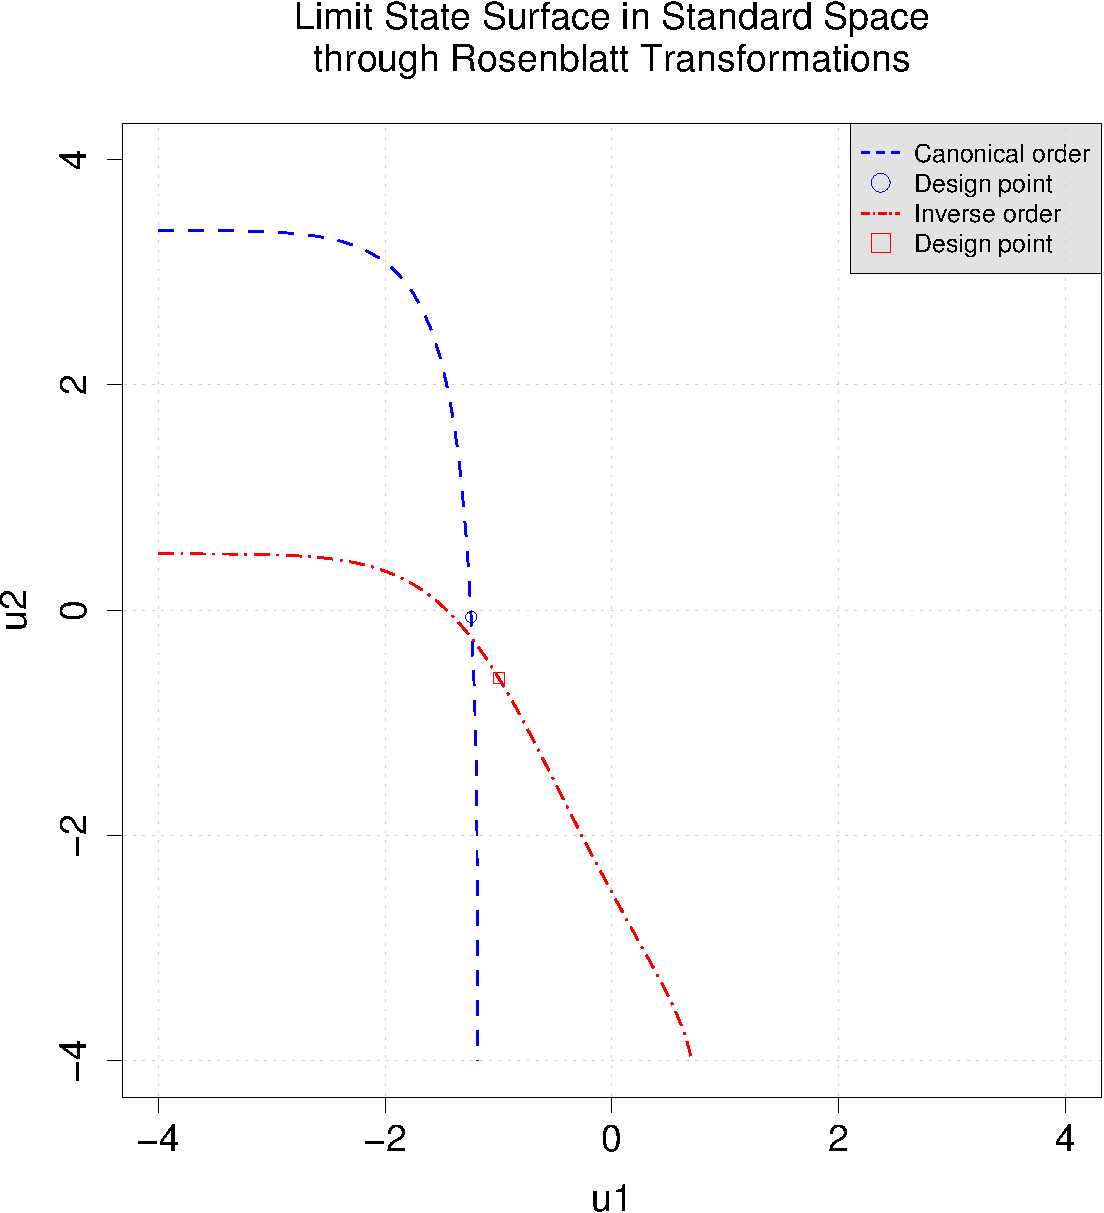
\includegraphics[height=7cm]{Figures/Final_SEL_ex2_marginExp.pdf}
              \end{center}



            }
